\vspace*{-5mm}
\mysection{Overall Description}

\mysubsection{Goals \& Requirements}
\vspace{0.2cm}
\mysubsubsection{EasyLib}
\vspace{0.5cm}
\noindent
\emph{\textbf{[G$_{1}$] : Allow the user to register and login into the system (also throughout external services)}}
\begin{itemize}
	\setlength{\leftskip}{0.5cm}
	\item \lbrack R$_{1}$] : The system has to check the credentials.
	\item \lbrack R$_{2}$] : A registered user must be able to log in the system.
	\item \lbrack R$_{3}$] : The System has to handle the connection and user requests.
	\item \lbrack R$_{4}$] : The system has to be able to save locally the user credentials to allow the automatic login.
	\item \lbrack R$_{5}$] : The system has to be able to communicate with the external services and receive the responses.
	\item \lbrack R$_{6}$] : The system has to be able to show to the user his profile information.
\end{itemize}

\vspace{0.5cm}
\noindent
\emph{\textbf{[G$_{2}$] : Allow the user to select his favourite library}}
\begin{itemize}
	\setlength{\leftskip}{0.5cm}
	\item \lbrack R$_{1}$] : The system has to be able to check and retrieve libraries information from the DB.
	\item \lbrack R$_{2}$] : The system has to be able to recognize the libraries already set as favourite by the user.
	\item \lbrack R$_{3}$] : The system has to be able to set the preferred library selected by the user into the DB.
	\item \lbrack R$_{4}$] : The system has to be able to remove a library from the favourite libraries present in DB for the considered user.
	\item \lbrack R$_{5}$] : The system has to be able to show to the user his favourite libraries.
\end{itemize}

\vspace{0.5cm}
\noindent
\emph{\textbf{[G$_{3}$] : Allow the user to see all the libraries available into the system and their content}}
\begin{itemize}
	\setlength{\leftskip}{0.5cm}
	\item \lbrack R$_{1}$] : The system has to be able to retrieve library’s information and contents.
	\item \lbrack R$_{2}$] : The system has to be able to show the retrieved information and contents related to the libraries.
\end{itemize}

\newpage
\noindent
\emph{\textbf{[G$_{4}$] : Allow the user to search a book in the available libraries}}
\begin{itemize}
	\setlength{\leftskip}{0.5cm}
	\item \lbrack R$_{1}$] : The system has to be able to retrieve book’s information from the libraries using	title, author, genre and/or library name.
	\item \lbrack R$_{2}$] : The system has to be able to filter books using the book identifier, so it will show only one copy of the book even if it's present in more than one library.
	\item \lbrack R$_{3}$] : The system has to be able to show the book information to the user.
\end{itemize}

\vspace{0.5cm}
\noindent
\emph{\textbf{[G$_{5}$] : Allow user to retrieve book information through QRcode scan}}
\begin{itemize}
	\setlength{\leftskip}{0.5cm}
	\item \lbrack R$_{1}$] : The android app needs to have access to the camera sensor.
	\item \lbrack R$_{2}$] : The android app has to be able to decode the QRcode attached to the book.
	\item \lbrack R$_{3}$] : The system has to be able to retrieve book information using the identifier decoded.
\end{itemize}

\vspace{0.5cm}
\noindent
\emph{\textbf{[G$_{6}$] : Allow the user to receive notifications from the server}}
\begin{itemize}
	\setlength{\leftskip}{0.5cm}
	\item \lbrack R$_{1}$] : The Application Server has to be able to send notifications to the android app.
	\item \lbrack R$_{2}$] : The Android app as to be able to receive and handle incoming notifications.
	\item \lbrack R$_{3}$] : The Android app has to be able to show the notifications to the user.
\end{itemize}

\vspace{0.5cm}
\noindent
\emph{\textbf{[G$_{7}$] : Allow the user to reserve books}}
\begin{itemize}
	\setlength{\leftskip}{0.5cm}
	\item \lbrack R$_{1}$] : The System has to retrieve the information of the book status from the DB.
	\item \lbrack R$_{2}$] : The System has to be able to change the status of the book to reserved / not reserved.
	\item \lbrack R$_{3}$] : The System has to show to the user all the books that he reserved.
\end{itemize}

\vspace{0.5cm}
\noindent
\emph{\textbf{[G$_{8}$] : Allow the user to get in line for a book}}
\begin{itemize}
	\setlength{\leftskip}{0.5cm}
	\item \lbrack R$_{1}$] : The System has to retrieve the information of the book status from the DB.
	\item \lbrack R$_{2}$] : The System has to be able to change the status of the book to “on waiting list” / “not in waiting list”.
	\item \lbrack R$_{3}$] : The System has to show to the user all the books for which he is in line.
	\item \lbrack R$_{4}$] : The System has to be able to manage the waiting list flowing when some reservation related to the considered book is removed.
\end{itemize}

\vspace{0.5cm}
\noindent
\emph{\textbf{[G$_{9}$] : Allow the user to see the books that he read}}
\begin{itemize}
	\setlength{\leftskip}{0.5cm}
	\item \lbrack R$_{1}$] : The System has to be able to retrieve the books read from the user.
	\item \lbrack R$_{2}$] : The Android application has to be able to show the books read by the user.
\end{itemize}

\vspace{0.5cm}
\noindent
\emph{\textbf{[G$_{10}$] : Allow the user to rate a read book}}
\begin{itemize}
	\setlength{\leftskip}{0.5cm}
	\item \lbrack R$_{1}$] : The System has to be able to retrieve the books’ information.
	\item \lbrack R$_{2}$] : The System has to be able to recognize if the book has been read by the user.
	\item \lbrack R$_{3}$] : The System has to be able to insert the user rating into the DB.
	\item \lbrack R$_{4}$] : The DB has to be able to update the average rating after each rate insertion.
\end{itemize}

\vspace{0.5cm}
\noindent
\emph{\textbf{[G$_{11}$] : Allow the user to reserve a seat for an event}}
\begin{itemize}
	\setlength{\leftskip}{0.5cm}
	\item \lbrack R$_{1}$] : The System has to be able to retrieve the events from the DB.
	\item \lbrack R$_{2}$] : The System has to check the available seats.
	\item \lbrack R$_{3}$] : The System has to allow the user to insert his participation to the event in the DB.
	\item \lbrack R$_{4}$] : The System has to allow the user to remove his participation to the event in the DB.
	\item \lbrack R$_{5}$] : The Android application has to show to the user his status related to the participation to an event.
\end{itemize}

\vspace{0.5cm}
\noindent
\emph{\textbf{[G$_{12}$] : Allow the user to see all the events that he joined}}
\begin{itemize}
	\setlength{\leftskip}{0.5cm}
	\item \lbrack R$_{1}$] : The System has to be able to retrieve all the events joined by the considered user.
	\item \lbrack R$_{2}$] : The Android application has to be able to show the events joined by the user.
\end{itemize}

\newpage
\noindent
\emph{\textbf{[G$_{13}$] : Allow the user to edit his profile information}}
\begin{itemize}
	\setlength{\leftskip}{0.5cm}
	\item \lbrack R$_{1}$] : The Android application has to be able to show to the user his profile information.
	\item \lbrack R$_{2}$] : The System has to be able to retrieve the user’s profile information from the DB.
	\item \lbrack R$_{3}$] : The System has to be able to update user’s profile information into the DB.
\end{itemize}

\vspace{0.8cm}
\mysubsubsection{EasyLib - Librarian}
\vspace{0.5cm}
\noindent
\emph{\textbf{[G$_{1}$] : Allow the librarian to login into the system}}
\begin{itemize}
	\setlength{\leftskip}{0.5cm}
	\item \lbrack R$_{1}$] : The system has to check the credentials.
	\item \lbrack R$_{2}$] : Registered user must be able to log in the system.
	\item \lbrack R$_{3}$] : The system has to handle the connection and user requests.
	\item \lbrack R$_{4}$] : The system has to be able to show to the user his relative library information.
\end{itemize}

\vspace{0.5cm}
\noindent
\emph{\textbf{[G$_{2}$] : Allow librarian to retrieve book information through QRcode scan}}
\begin{itemize}
	\setlength{\leftskip}{0.5cm}
	\item \lbrack R$_{1}$] : The android app needs to have access to the camera sensor.
	\item \lbrack R$_{2}$] : The android app has to be able to decode the QRcode attached to the book.
	\item \lbrack R$_{3}$] : The system has to be able to retrieve the book information using the identifier decoded.
\end{itemize}

\vspace{0.5cm}
\noindent
\emph{\textbf{[G$_{3}$] : Allow the librarian to confirm/remove reservations for a specific book}}
\begin{itemize}
	\setlength{\leftskip}{0.5cm}
	\item \lbrack R$_{1}$] : The system has to be able to retrieve the reservation list for a book.
	\item \lbrack R$_{2}$] : The system has to be able to get the librarian input and change the reservation status of a book.
\end{itemize}

\vspace{0.5cm}
\noindent
\emph{\textbf{[G$_{3}$] : Allow the librarian to communicate to the system when a book is returned}}
\begin{itemize}
	\setlength{\leftskip}{0.5cm}
	\item \lbrack R$_{1}$] : The system has to be able to retrieve book information and check its status.
	\item \lbrack R$_{2}$] : The system has to be able to trigger the insert in the reservation list of the requests in waiting list and send them a notification.
\end{itemize}

\mysubsubsection{EasyLib - Librarian (Future Work)}
\vspace{0.5cm}
\noindent
\emph{\textbf{[FW$_{1}$] : Allow the librarian to register into the system.}}

\vspace{0.5cm}
\noindent
\emph{\textbf{[FW$_{2}$] : The system has to be able to save locally the librarian credentials to allow the automatic login.}}

\vspace{0.5cm}
\noindent
\emph{\textbf{[FW$_{3}$] : Allow the librarian to search for a book in his library.}}

\vspace{0.5cm}
\noindent
\emph{\textbf{[FW$_{4}$] : Allow the librarian to edit library information.}}

\vspace{0.5cm}
\noindent
\emph{\textbf{[FW$_{5}$] : Allow the librarian to change library contents (add/remove news, events and books).}}

\vspace{0.5cm}
\mysubsection{Product Functions}
\vspace{0.5cm}
\mysubsubsection{EasyLib}
\vspace*{0cm}
\begin{figure}[H]
	\centering
	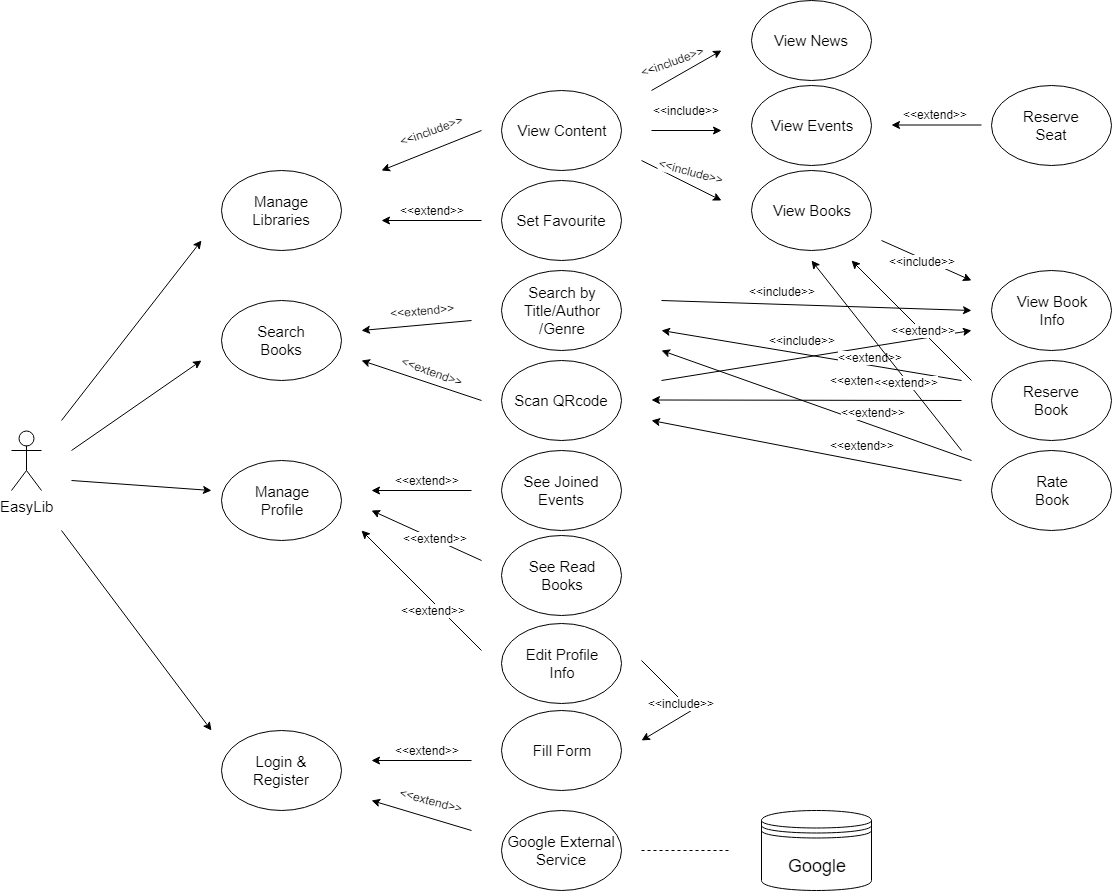
\includegraphics[scale=0.4]{Images/UseCases/EasyLib_use_case}
	\caption{EasyLib - Use Case}
\end{figure}
\begin{enumerate}
\item \emph{Advanced book search:}the user can search a book in the libraries using any combination of parameters between title, author’s name and category and, if he needs, he can also restrict his search in only one of the available libraries. If the user is in the library, he can scan a QR code on the book to retrieve all its information.
\item \emph{Consulting book information:} the user can consult all the available book’s information such as title, author’s name, the number of copies of the book available in each library, etc.
\item \emph{Reserve or get in line for a book:} the user can reserve a copy of the book if available or get in line for it just tapping a bottom.
\item \emph{Visualize libraries’ news and events:}the user can remain constantly up-to-date with the new events organized and news posted by the available libraries checking out their dedicated pages. 
\item \emph{Book a seat to an event:} : the user can book a seat in the events organized by the libraries to avoid the risk of missing the meeting with his favourite authors.
\item \emph{Save favourite libraries:} the user can select his favourite libraries between that ones present on the system in order to have a rapid access to their books, events and news. 
\item \emph{Set ratings:} the user can rate the books that he has read to spread his opinion to other readers.
\item \emph{Keep track of read books:} the user can always access to the list of the book that he read directly and intuitively from his profile.
\end{enumerate}

\newpage
\mysubsubsection{EasyLib - Librarian}
\begin{figure}[H]
	\centering
	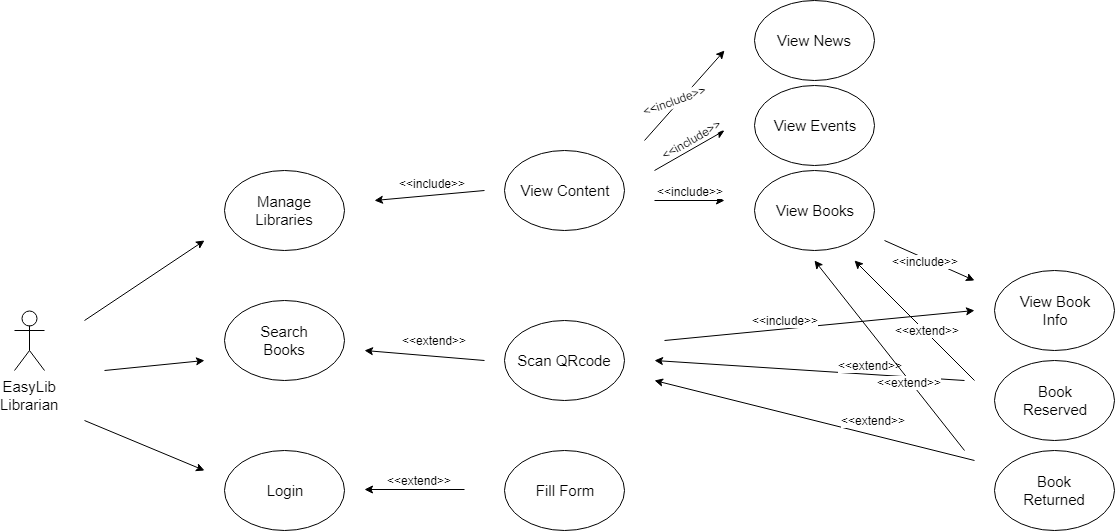
\includegraphics[scale=0.4]{Images/UseCases/EasyLib_Librarian_use_case}
	\caption{EasyLib - Librarian - Use Case}
\end{figure}
\begin{enumerate}
\item \emph{Visualize his library information:}the librarian can visualize all the information inserted in his library such as books available, events, news, etc.
\item \emph{Identify the user that reserved a book:} the librarian can scan the QRcode of a book and retrieve all the reservation for that book and the related user id. In this way the user can show to the librarian his personal Id authenticating himself and allowing the book delivering. A paired process is followed when the user returns a book.
\item \emph{Record that a user has returned a book:} with the same approach of the former feature, the librarian can update into the Database a book status to returned.
\end{enumerate}


\mysubsection{Domanin Properties}
In order to have the aimed behaviour of the app, few domain constraints must be satisfied.

\begin{itemize}
	\item The user needs to have a mobile phone or a tablet that support Android OS.
	\item The Android OS version installed on the device must be KitKat (API level 19) or higher.
	\item An access to an internet connection is always needed.
	\item The users must be able to easily reach the physical library location to use the functionalities that need an interaction with the librarians, such as take and return a reserved book.
\end{itemize}